\section{\bf Conclusion}\label{sec:conclusion}
The creation of a reliable humanoid throwing method was completed. 
This allowed the Hubo to complete its goal of becoming the first full-size humanoid to throw the first pitch at a Major League Baseball game.
Anthropomorphizing the robotic pitch was done via outfitting Jaemi with a uniform shirt and cap.
Hubo also gestured to the crowd via waving during its entrance and exit of the field to further engage the audience at the \textit{Science Night at the Ballpark}.
Three methods of creating a viable pitch were explored and tested: (1) human-robot mapping via motion capture, (2) sparse reachable map based trajectory generation and (3) a key-frame based method.  
Though the key-frame based method was the simplest it also proved to be the most viable.  
The balancing controller ensured stability of the system throughout the throw.  
The addition of a high powered wrist and having the robot step forward when it throws created conditions for a successful and reliable pitch.
The latter methods answered the challenges posed in the area of full-body locomotion, coordination and stabilization.

Prior full-size humanoid throwing methods such as the work by Kim et al. \cite{5686315} were only shown in simulation.
This paper's set of experiments and demonstrations shows the realization of these same tasks in the physical world.
Throughout all of the experiments the system was manually aimed prior to each pitch.
Each of the robot's pitches are accurate however a key factor in off-target or \textit{wild} pitches is improper aiming during setup.
The addition of feedback via a targeting system similar to that of Hu et al.~\cite{5649335} would remove the need for manual targeting of the robot and will be incorporated in the next revision of the pitching Hubo.

\begin{figure}[t]
  \centering
  
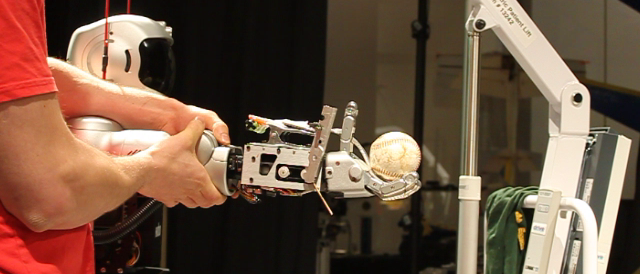
\includegraphics[width=0.5\columnwidth]{./pix/arm0.png}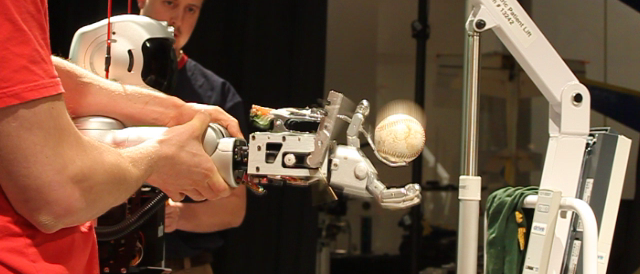
\includegraphics[width=0.5\columnwidth]{./pix/arm1.png}
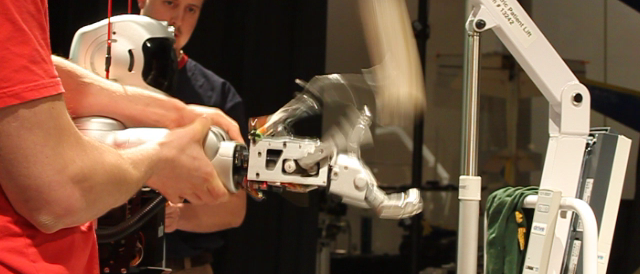
\includegraphics[width=0.5\columnwidth]{./pix/arm2.png}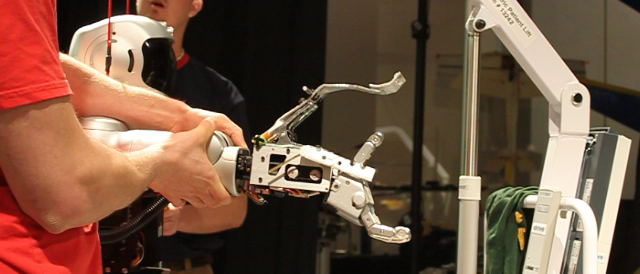
\includegraphics[width=0.5\columnwidth]{./pix/arm3.png}
%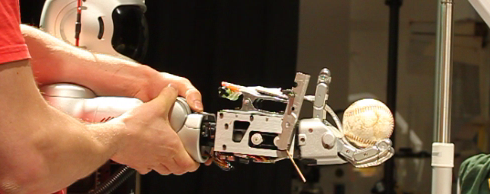
\includegraphics[width=0.6\columnwidth]{./pix/finalSpring1.png}
%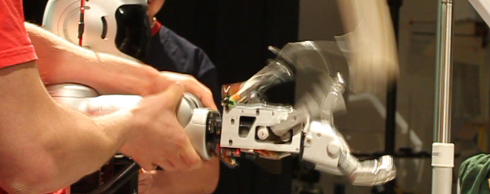
\includegraphics[width=0.6\columnwidth]{./pix/finalSpring2.png}
%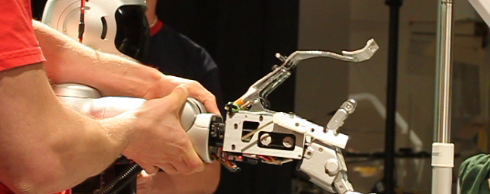
\includegraphics[width=0.6\columnwidth]{./pix/finalSpring3.png}
  \caption{Spring loaded mechanism test launching the baseball.  Top-Left: Pre-launch.  Top-Right/Bottom-Left: Launch.  Bottom-Right: Pos-launch.  The mechanism added 3.0 $\frac{m}{s}$ to the end-effector velocity at its release point.}
  \label{fig:hubo-spring}
\end{figure}

This work is a step towards full-size humanoids performing fast and accurate full body tasks.
Though one might perceive robots to be \textit{better} than people (faster, more accurate, etc.) the reality is that the field of humanoid robotics is still in its infant state and Hubo is only the size of a ten year old child.
Having Hubo complete this task shows that full-size humanoids can perform some tasks at a ten year old's level.
More information and media about this event is available on this papers home page http://danlofaro.com/urai2012/



%In in completing this challenge the overarching fields of fully  

%of full body locomotion/coordination and stability were addressed.









%The challenges in completing this task included full body locomotion, stabilization, 